%
% This is a borrowed LaTeX template file for lecture notes for CS267,
% Applications of Parallel Computing, UCBerkeley EECS Department.
% Now being used for CMU's 10725 Fall 2012 Optimization course
% taught by Geoff Gordon and Ryan Tibshirani.  When preparing 
% LaTeX notes for this class, please use this template.
%
% To familiarize yourself with this template, the body contains
% some examples of its use.  Look them over.  Then you can
% run LaTeX on this file.  After you have LaTeXed this file then
% you can look over the result either by printing it out with
% dvips or using xdvi. "pdflatex template.tex" should also work.
%

\documentclass[twoside]{article}
\setlength{\oddsidemargin}{0.25 in}
\setlength{\evensidemargin}{-0.25 in}
\setlength{\topmargin}{-0.6 in}
\setlength{\textwidth}{6.5 in}
\setlength{\textheight}{8.5 in}
\setlength{\headsep}{0.75 in}
\setlength{\parindent}{0 in}
\setlength{\parskip}{0.1 in}

%
% ADD PACKAGES here:
%

\usepackage{amsmath,amsfonts,graphicx}

%
% The following commands set up the lecnum (lecture number)
% counter and make various numbering schemes work relative
% to the lecture number.
%
\newcounter{lecnum}
\renewcommand{\thepage}{\thelecnum-\arabic{page}}
\renewcommand{\thesection}{\thelecnum.\arabic{section}}
\renewcommand{\theequation}{\thelecnum.\arabic{equation}}
\renewcommand{\thefigure}{\thelecnum.\arabic{figure}}
\renewcommand{\thetable}{\thelecnum.\arabic{table}}

%
% The following macro is used to generate the header.
%
\newcommand{\lecture}[4]{
   \pagestyle{myheadings}
   \thispagestyle{plain}
   \newpage
   \setcounter{lecnum}{#1}
   \setcounter{page}{1}
   \noindent
   \begin{center}
   \framebox{
      \vbox{\vspace{2mm}
    \hbox to 6.28in { {\bf EE302 - Feedback Systems
	\hfill Spring 2018} }
       \vspace{4mm}
       \hbox to 6.28in { {\Large \hfill Lecture #1 \hfill} }
       \vspace{2mm}
       \hbox to 6.28in { {\it Lecturer: #2 \hfill } }
      \vspace{2mm}}
   }
   \end{center}
   \markboth{Lecture #1}{Lecture #1}

   \vspace*{4mm}
}
%
% Convention for citations is authors' initials followed by the year.
% For example, to cite a paper by Leighton and Maggs you would type
% \cite{LM89}, and to cite a paper by Strassen you would type \cite{S69}.
% (To avoid bibliography problems, for now we redefine the \cite command.)
% Also commands that create a suitable format for the reference list.
\renewcommand{\cite}[1]{[#1]}
\def\beginrefs{\begin{list}%
        {[\arabic{equation}]}{\usecounter{equation}
         \setlength{\leftmargin}{2.0truecm}\setlength{\labelsep}{0.4truecm}%
         \setlength{\labelwidth}{1.6truecm}}}
\def\endrefs{\end{list}}
\def\bibentry#1{\item[\hbox{[#1]}]}

%Use this command for a figure; it puts a figure in wherever you want it.
%usage: \fig{NUMBER}{SPACE-IN-INCHES}{CAPTION}
\newcommand{\fig}[3]{
			\vspace{#2}
			\begin{center}
			Figure \thelecnum.#1:~#3
			\end{center}
	}
% Use these for theorems, lemmas, proofs, etc.
\newtheorem{theorem}{Theorem}[lecnum]
\newtheorem{lemma}[theorem]{Lemma}
\newtheorem{proposition}[theorem]{Proposition}
\newtheorem{claim}[theorem]{Claim}
\newtheorem{corollary}[theorem]{Corollary}
\newtheorem{definition}[theorem]{Definition}
\newenvironment{proof}{{\bf Proof:}}{\hfill\rule{2mm}{2mm}}

% **** IF YOU WANT TO DEFINE ADDITIONAL MACROS FOR YOURSELF, PUT THEM HERE:

\begin{document}

% Lecture Details
\lecture{9}{Asst. Prof. M. Mert Ankarali}
....

\section{Steady-Sate Response Analysis}

Fundamental concept that we need to perform
stead-state response analysis of a control
system is the final value theorem. Given a continuous time signal 
$x(t)$ and its Laplace transform $X(s)$, if $x(s)$ is convergent signal,
final value theorem states that
%
\begin{align*}
\lim_{t\to \infty} x(t) &= \lim_{s \to 0} \left[ s X(s) \right]
\\
x_{ss} &= \lim_{s \to 0} \left[ s X(s) \right]
\end{align*}

\subsection{Tracking Performance}

The most important steady-state performance 
condition for a control system is the tracking performance
under steady-state conditions. Let's consider the
following fundamental feedback topology. 

    \begin{center}
\begin{minipage}[h]{0.8\linewidth}
    \begin{center}
      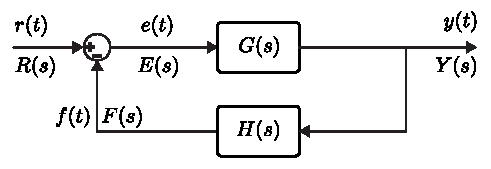
\includegraphics[width=\textwidth]{feedback}
    \end{center}
\end{minipage}
    \end{center}

In order to achieve a good tracking performance, obviously 
the error signal $e(t)$ need to be small. Accordingly, steady-state 
tracking performance is determined by the steady-state error
of the closed-loop system, that we can compute using final
value theorem as
%
\begin{align*}
	e_{ss} = \lim_{t\to \infty} e(t) &= \lim_{s \to 0} \left[ s e(s) \right]
\end{align*}
%
Let's compute $E(s)/R(s)$, i.e. transfer function from the reference input to the 
error signal, 
%
\begin{align*}
E(s) &= R(s) - E(s) G(s) H(s)  , 
\\
\frac{E(s)}{R(s)} &= \frac{1}{1 + G(s) H(s) }
\end{align*}
%
Note that $G(s) H(s)$ is the  transfer function from the error
signal $E(s)$ to the signal which is fed to the negative terminal of 
the main difference operator, i.e. $F(s)$. This transfer function is
called the feed-forward or open-loop  pulse transfer function of the 
closed-loop dcontrol system. For this system, 
%
\begin{align*}
\frac{F(s)}{E(s)} = G_{OL} = G(s) H(s)
\end{align*}
%
Then $E(s)$ can be written as
%
\begin{align*}
E(s) = R(s) \frac{1}{1 + G_{OL} (s) }
\end{align*}
%
It is obvious that first requirement on steady-state error
performance is that closed-loop system have to be stable.
Now let's analyze specific but fundamental input scenarios. 

\subsection*{Unit-Step Input}

We know that $r(t) = h(t)$ and $R(s) = \frac{1}{s}$ then 
we have
%
\begin{align*}
e_{ss} &= \lim_{s \to 0} \left[ s R(s) \frac{1}{1
         + G_{OL} (s) } \right]
\\
&= \lim_{s \to 0} \left[ s \frac{1}{s} \frac{1}{1
         + G_{OL} (s) } \right]
\\
e_{ss} &= \frac{1}{1 + \lim_{s \to 0} G_{OL} (s) }
\end{align*}
%
If the DC gain of the system (also called static error constant) is
constant, i.e. $\lim_{s \to 0}G_{OL}(s) = K_{DC}$ then the steady state error can be
computed as
%
\begin{align*}
e_{ss} &= \frac{1}{1 + K_{DC}}
\end{align*}
%
It is obvious that 
%
\begin{align*}
e_{ss} &\neq 0 \quad \mathrm{if} \quad |K_{DC}| < \infty
\\
e_{ss} &\to 0 \quad \mathrm{if} \quad K_{DC} \to \infty
\end{align*}
%
At this point, it could be helpful to introduce the concept of system \textit{type},
to generalize the steady-state error analysis. 

\textbf{Definition:} Let's write the open-loop transfer function of a closed-loop
system in the following standard form
%
\begin{align*}
G_{OL}(s) = \frac{K}{s^N} \frac{b_0 s^m + \cdots + b_{m-1} s + 1}{a_0 s^n + \cdots + a_{n-1} s + 1}
\end{align*}
%
The closed-loop system is called as \textbf{Type N} system, where
$N$ is the $\#$ if integrators in the open-loop transfer function (OLTF).

Based on these results, we can have the following conclusions
regarding steady-state error for unit-step input
%
\begin{itemize}
\item If $G_{OL} (0) = K_P$ , $| K_{P} | < \infty$, then 
\begin{align*}
e_{ss} =1/(1 + K_{P})
\end{align*}
% 
These are \textbf{Type 0} (or \textbf{Type $N \leq 0$})
systems. We observe a bounded steady-state error and it is possible to reduce the error by increasing the static gain
constant $K_P$. 
%
\item  If $G_{OL} (0) = \infty$, then $e_{ss} = 0$. In other words, for 
  \textbf{Type $N > 0$} systems, the steady-state error is perfectly zero .
\end{itemize}

Now let's summarize the steady-state error conditions
%
\begin{itemize}
\item Type $N \leq 0$: $e_{ss} =  \frac{1}{1 + K_{P}}$
\item Type $N > 0$: $e_{ss} = 0$
\end{itemize}

\subsection*{Unit-Ramp Input}
%
We know that $r(t) = t h(t)$ and $R(s) = \frac{1}{(s^2}$ then
we have

\begin{align*}
e_{ss} &= \lim_{s \to 0} \left[ s R(s) \frac{1}{1
         + G_{OL} (s) } \right]
\\
&= \lim_{s \to 0} \left[ s \frac{1}{s^2} \frac{1}{1
         + G_{OL} (s) } \right]
\\
 &= \frac{1}{lim_{s \to 0} s^{-1} G_{OL} (s) }
\\
e_{ss} &= \frac{1}{lim_{s \to 0} \frac{K}{s^{N-1}} \frac{b_0 s^m + \cdots + b_{m-1} s + 1}{a_0 s^n + \cdots + a_{n-1} s + 1} }
\end{align*}
%
Based on this result we can have the following steady-state
error conditions for the unit-ramp input based on the type 
condition of the system
%
\begin{itemize}
\item Type $N < 1$: $e_{ss} \to  \infty$
\item Type $N = 1$: $e_{ss} = \frac{1}{K_v}$
\item Type $N > 1$: $e_{ss} = 0$
\end{itemize}
%
where $K_v$ is called the static velocity error constant.
 
\subsection*{Unit-Quadratic (Acceleration) Input}
%
We know that $r(t) = \frac{1}{2} t^2 h(t)$ and $R(s) = \frac{1}{s^3}$ then
we have
\begin{align*}
e_{ss} &= \lim_{s \to 0} \left[ s R(s) \frac{1}{1
         + G_{OL} (s) } \right]
\\
&= \lim_{s \to 0} \left[ s \frac{1}{s^3} \frac{1}{1
         + G_{OL} (s) } \right]
\\
 &= \frac{1}{lim_{s \to 0} s^{-2} G_{OL} (s) }
\\
e_{ss} &= \frac{1}{lim_{s \to 0} \frac{K}{s^{N-2}} \frac{b_0 s^m + \cdots + b_{m-1} s + 1}{a_0 s^n + \cdots + a_{n-1} s + 1} }
\end{align*}
%
Based on this result we can have the following steady-state
error conditions for the unit-ramp input based on the type 
condition of the system
%
\begin{itemize}
\item Type $N < 2$: $e_{ss} \to  \infty$
\item Type $N = 2$: $e_{ss} = \frac{1}{K_{a}}$
\item Type $N > 2$: $e_{ss} = 0$
\end{itemize}
%
where $K_v$ is called the static acceleration error constant.

\paragraph{Example 1:} Compute the $G_{OL}(s)$ for the following closed-loop
system and define its \textbf{Type}. After that, compute the steady-state errors to unit-step, unit-ramp, a
and unit-quadratic inputs.

\begin{center}
\begin{minipage}[h]{0.75\linewidth}
    \begin{center}
      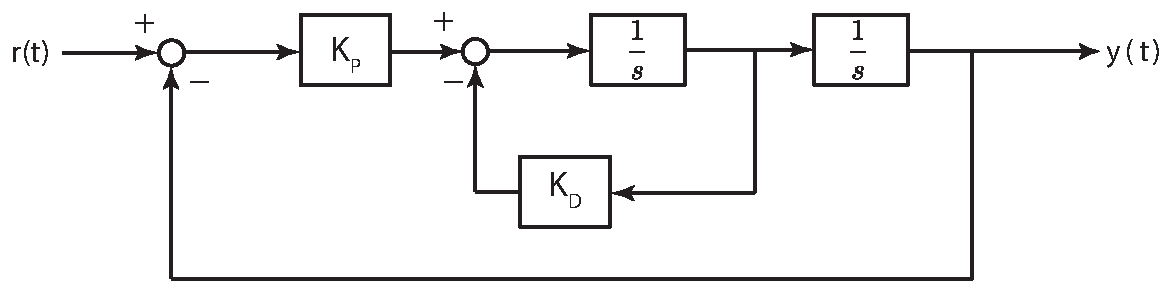
\includegraphics[width=\textwidth]{example}
    \end{center}
\end{minipage}
\end{center}

\paragraph{Solution:} 
%
\begin{align*}
&G_{OL}(s) =  \frac{K_P}{s ( s + K_D)} 
\\
&\mathrm{Type} \ 1  \quad, \ K_v = \frac{K_P}{K_D}
\end{align*}
%
Then the steady-state errors are computed as
\begin{itemize}
\item Unit-step: $e_{ss} = 0$
\item Unit-ramp: $e_{ss} = \frac{K_D}{K_P}$
\item Unit-acceleration: $e_{ss} = \infty$
\end{itemize}

\paragraph{Example 2:} Compute the $G_{OL}(s)$ for the following closed-loop
system and define its \textbf{Type}. After that, compute the steady-state errors to unit-step, unit-ramp, a
and unit-quadratic inputs.

\begin{center}
\begin{minipage}[h]{0.75\linewidth}
    \begin{center}
      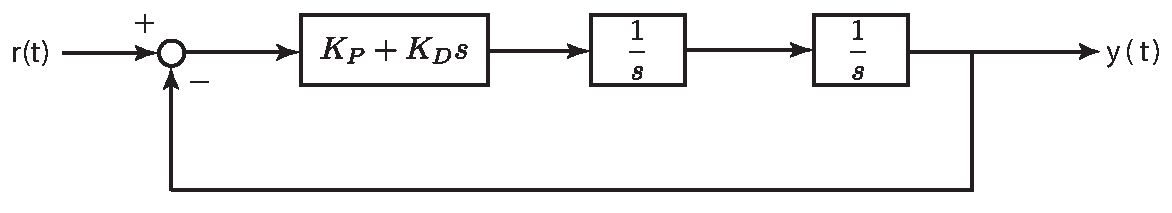
\includegraphics[width=\textwidth]{example2}
    \end{center}
\end{minipage}
\end{center}

\paragraph{Solution:} 
%
\begin{align*}
&G_{OL}(s) =  \frac{K_P + K_D s}{s^2} 
\\
&\mathrm{Type} \ 2  \quad, \ K_a = K_P
\end{align*}
%
Then the steady-state errors are computed as
\begin{itemize}
\item Unit-step: $e_{ss} = 0$
\item Unit-ramp: $e_{ss} = 0$
\item Unit-acceleration: $e_{ss} = \frac{1}{K_a}$
\end{itemize}


\paragraph{Example 3:} Compute the $G_{OL}(s)$ for the following closed-loop
system and define its \textbf{Type}. After that, compute the steady-state errors to unit-step, unit-ramp, a
and unit-quadratic inputs.

\begin{center}
\begin{minipage}[h]{0.6\linewidth}
    \begin{center}
      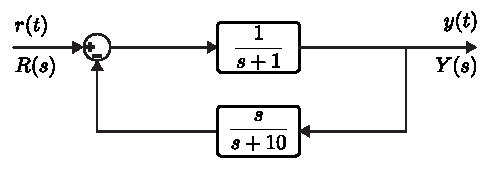
\includegraphics[width=\textwidth]{example3}
    \end{center}
\end{minipage}
\end{center}

\paragraph{Solution:} 
%
\begin{align*}
&G_{OL}(s) =  \frac{s}{(s+1) (s+10)} 
\\
&\mathrm{Type} \ \mathbf{-1}  \quad, \ K_P = 0
\end{align*}
%
Then the steady-state errors are computed as
\begin{itemize}
\item Unit-step: $e_{ss} = 1$
\item Unit-ramp: $e_{ss} = \infty$
\item Unit-acceleration: $e_{ss} = \infty$
\end{itemize}

\paragraph{Example 4:} Compute the steady-state error to unit-step input
for the following system. 

\begin{center}
\begin{minipage}[h]{0.75\linewidth}
    \begin{center}
      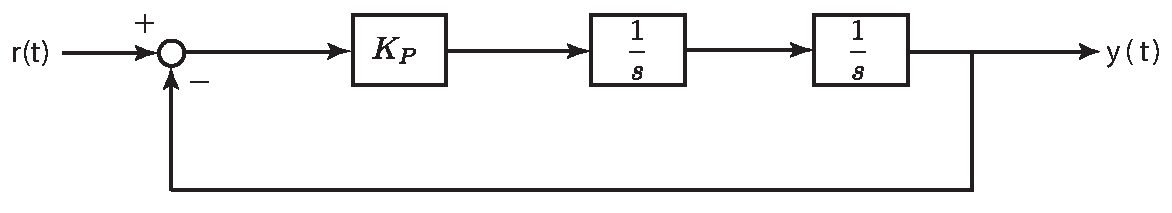
\includegraphics[width=\textwidth]{marginal}
    \end{center}
\end{minipage}
\end{center}

\paragraph{Bad Solution:}
%
\begin{align*}
&G_{OL}(s) =  \frac{K_p}{s^2} 
\\
&\mathrm{Type} \ \mathbf{2}  
\\
&e_{ss} = 0 \quad ??????
\end{align*}
%
\paragraph{Good Solution:}
%
Let's compte $Y(s)$ and then $y(t)$,
%
\begin{align*}
  Y(s) &= \frac{\frac{K_p}{s^2}}{1 + \frac{K_p}{s^2}} R(s) =
         \frac{K_p}{s (s^2 + K_p)} 
\\
 y(t) &= 1 - \cos (K t) \ t > 0
\end{align*}
%
Error function takes the form $e(t) = \cos (K t)$ which does not
have a limit, i.e., there is no $e_{ss}$. If closed-loop transfer
function has poles on imaginary axis then, we can not apply
final value theorem. 

\paragraph{Example 5:} Compute the steady-state error to unit-step input
for the following system when $K_P = 1$. 

\begin{center}
\begin{minipage}[h]{0.75\linewidth}
    \begin{center}
      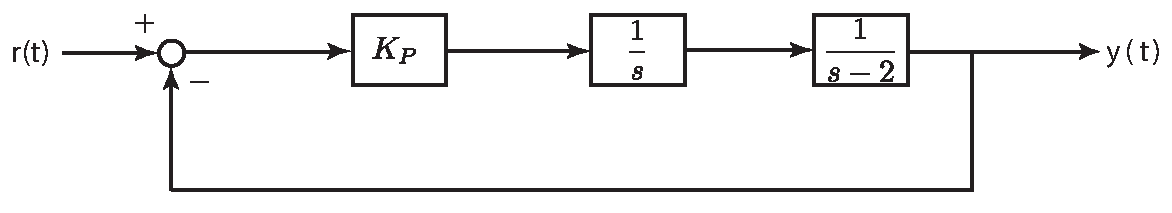
\includegraphics[width=\textwidth]{unstable}
    \end{center}
\end{minipage}
\end{center}

\paragraph{Good Solution :)} Let's check if $y(t)$ is a convergent
signal
%
%
\begin{align*}
  Y(s) &= \frac{\frac{1}{s (s-2)}}{1 + \frac{1}{s (s-2)}} R(s) =
         \frac{1}{s (s^2 - 2s + 1) } 
\\
 y(t) &= t e^t - e^t + 1 \ t > 0
\end{align*}
%
Error function takes the form $e(t) = e^t - t e^t$, thus 
%
\begin{align*}
 e_{ss} = | \lim_{t \to \infty} e(t) | = \infty 
\end{align*}
%
In conclusion, If closed-loop transfer function has poles on imaginary
axis or open right half-plane then, we can not apply final value theorem. 

\newpage

\subsection{Stead-State Response to Disturbances}

When analyzing the steady-state response of a system in addition to
the desired response to the reference input, it is also important
to analyze the response to unwanted disturbances and noises. 

Let's analyze the steady-state performance of the following 
topology which is perturbed by a disturbance input, $d(t)$. 

\begin{center}
\begin{minipage}[h]{0.75\linewidth}
    \begin{center}
      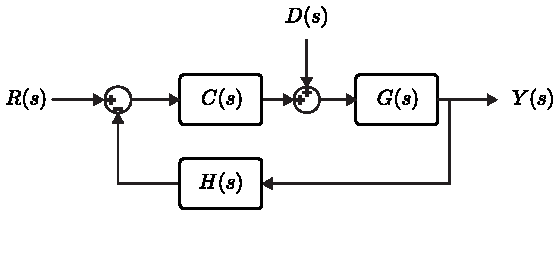
\includegraphics[width=\textwidth]{disturb}
    \end{center}
\end{minipage}
\end{center}

In order to analyze the response to the disturbance $d(t)$, we assume 
$r(t) = 0$ (which is just fine due to the linearity). Let's first find
the pulse transfer function from $D(s)$ to $Y(s)$. 
%
\begin{align*}
T_D(s) &= \frac{Y(s)}{D(s)} =  \frac{G(s)}{1 + C(s) G(s) H(s)}
\\
&= \frac{G(s)}{1 + G_{OL}(s)}
\end{align*}
%
Note that $Y(s)$ depends on both $G_{OL}(s)$ (OLTF) and $G(s)$ (Plant TF). 
If one wants to generalize the stead-state disturbance rejection performance,
he/she needs to analyze the conditions for both $G_{OL}(s)$ and $G(s)$. Moreover,
for a different topology and type of disturbance, we can have very different conditions. 
For this reason, in order to analyze steady-state disturbance/noise rejection
performance, it is better to use fundamentals and apply final value theorem.

\newpage

\paragraph{Example 6:} The following closed-loop system
is affected by a disturbance input $d(t)$. Compute the 
steady-state performance/response to a unit step disturbance 
input.

\begin{center}
\begin{minipage}[h]{0.8\linewidth}
    \begin{center}
      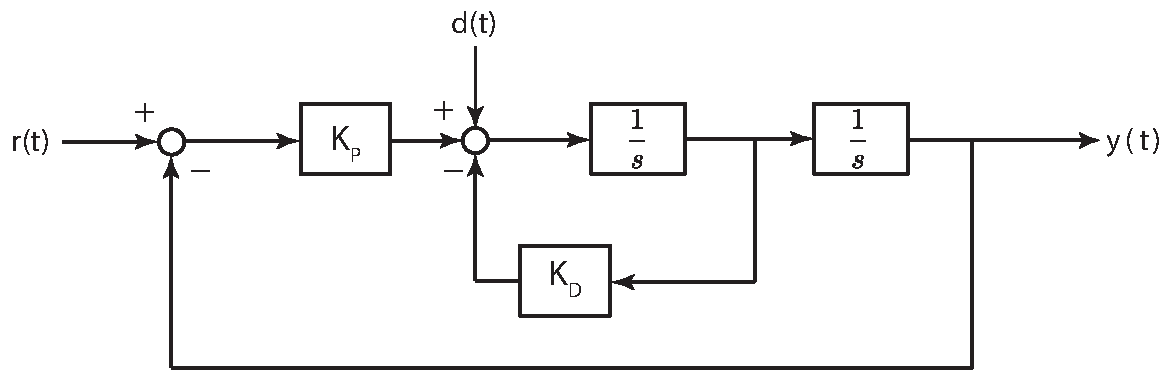
\includegraphics[width=\textwidth]{example4}
    \end{center}
\end{minipage}
\end{center}

\paragraph{Solution:} Lets compute $Y(s)/D(s)$
%
\begin{align*}
Y(s) &= \left( D(s) - Y(s) K_P \right) \frac{1}{s(s + K_D)} 
\\
Y(s) \left[ 1 + \frac{K_P}{s(s + K_D)}  \right] &= D(s) \frac{1}{s(s + K_D)} 
\\
\frac{Y(s)}{D(s)} &= \frac{\frac{1}{s(s + K_D)} }{\frac{s^2 + K_D s + K_P}{s(s + K_D)}}
= \frac{1}{s^2 + K_D s + K_P}
\end{align*}
%
 Now let's compute $y_{ss}$,
 %
 \begin{align*} 
y_{ss} &= \lim_{s \to 0} [ s Y(s) ] = \lim_{s \to 0} \left[ s D(s) \frac{1}{s^2 + K_D s + K_P} \right]  
\\
&= \lim_{s \to 0} \left[ s \frac{1}{s} \frac{1}{s^2 + K_D s + K_P} \right]  
\\
&= \frac{1}{K_P}
 \end{align*}
%
We can see that even if same system has 0 steady-state error when the reference
signal is step-like input, the error under unit-step disturbance is not zero, i.e., $y_{ss} = 1 / K_P$.
One can improve the disturbance rejection performance by increasing the $K_P$ gain. 


% **** This ENDS THE EXAMPLES. DON'T DELETE THE FOLLOWING LINE:
\end{document}